% !TeX root = ../main.tex

\chapter{系统设计与实现}\label{figures_tables}
第三、四章分别对本文提出的“基于神经辐射场的快速新视图合成方法”的方法论的详述和在公开数据集上大量的实验对比验证。为了将上述研究方法转成实际的系统,本文设计并实现了基于神经辐射场的快速新视图合成系统。此系统可以接入移动端三维传感器采集的多视角的图像,再通过本文提出的方法训练出高保真的神经辐射场,最终可以快速渲染出任意新视角的视图,可以和已知位姿的 ground truth 进行对比。

\section{系统需求分析}

\subsection{功能性需求分析}
基于上一节提出的系统设计的思路,本文基于神经辐射场的新视图快速合成系统可分为两大模块,分别是数据处理模块和算法模块,具体见图~\ref{fig:system_struct}。
\begin{figure}[htbp]
    \centering
    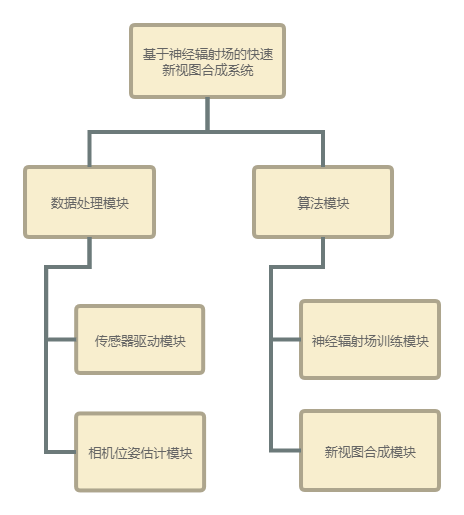
\includegraphics[width=0.65\linewidth]{figures/system_struct.png}
    \caption{系统架构图}
    \label{fig:system_struct}
\end{figure}

\begin{enumerate}
    \item [a)] 数据处理模块:包括以下两个模块内容:
               \begin{enumerate}
                   \item [1)] 传感器驱动模块:用于获取传感器的数据,例如 RGB 图像。
                   \item [2)] 相机位姿估计模块:使用 COLMAP \cite{schonberger2016structure} 实现对真实图像位姿的计算。
               \end{enumerate}
    \item [b)] 算法模块:包括以下两个模块内容:
               \begin{enumerate}
                   \item [1)] 神经辐射场训练模块:用于将已知位姿的图像训练成一个 5D 神经辐射场。
                   \item [2)] 新视图合成模块:通过训练好的模型,给定位姿,合成该位姿下的新视图。
               \end{enumerate}        
\end{enumerate}

\subsection{其他需求分析}
在经典的软件质量模型 “FURPS+” 中,除了上一小节的功能性需求,还剩下四个非功能性需求,分别是易用性 (Usability)、可靠性 (Reliability)、性能 (Performance) 还有可支持性 (Supportability)。使用 “FURPS+” 模型来实现需求分析可保障用户体验,比较好地能保证系统的运行质量。

以下是对本系统的非功能性需求进行分析:
\begin{enumerate}
    \item [a)] 易用性:在设计该系统的时候,系统的界面应该整洁美观,按钮名称应该通俗易懂,符合用户的操作习惯,降低用户的学习成本。
    \item [b)] 可靠性:系统应该足够鲁棒,能够处理各个模块中可能产生的异常,尽可能避免系统崩溃,如出现不可避免的错误应及时反馈给用户。     
    \item [c)] 性能:系统应在相关的平台上能流畅运行,系统的时延要能满足一般用户体验,本身应增加与用户交流的对话框,提高用户体验。此外,性能还体现在合成新视图的速度以及质量上,这是本文方法论所主要考量的指标。
    \item [d)] 可支持性:系统各功能模块清晰明确,模块之间应该是解耦的,方便日后维护、扩展、更新。接口命名以及教程足够清晰,方便其他开发者使用。
\end{enumerate}

\subsection{主要用例分析}
本小节主要介绍 PC 端的各个应用模块用例。

用户可以进行的操作包括与相机的交互,数据集的处理,以及新视图合成。用例图见图~\ref{fig:PCusercase}。

\pagebreak
\begin{figure}[htb]
	\centering
	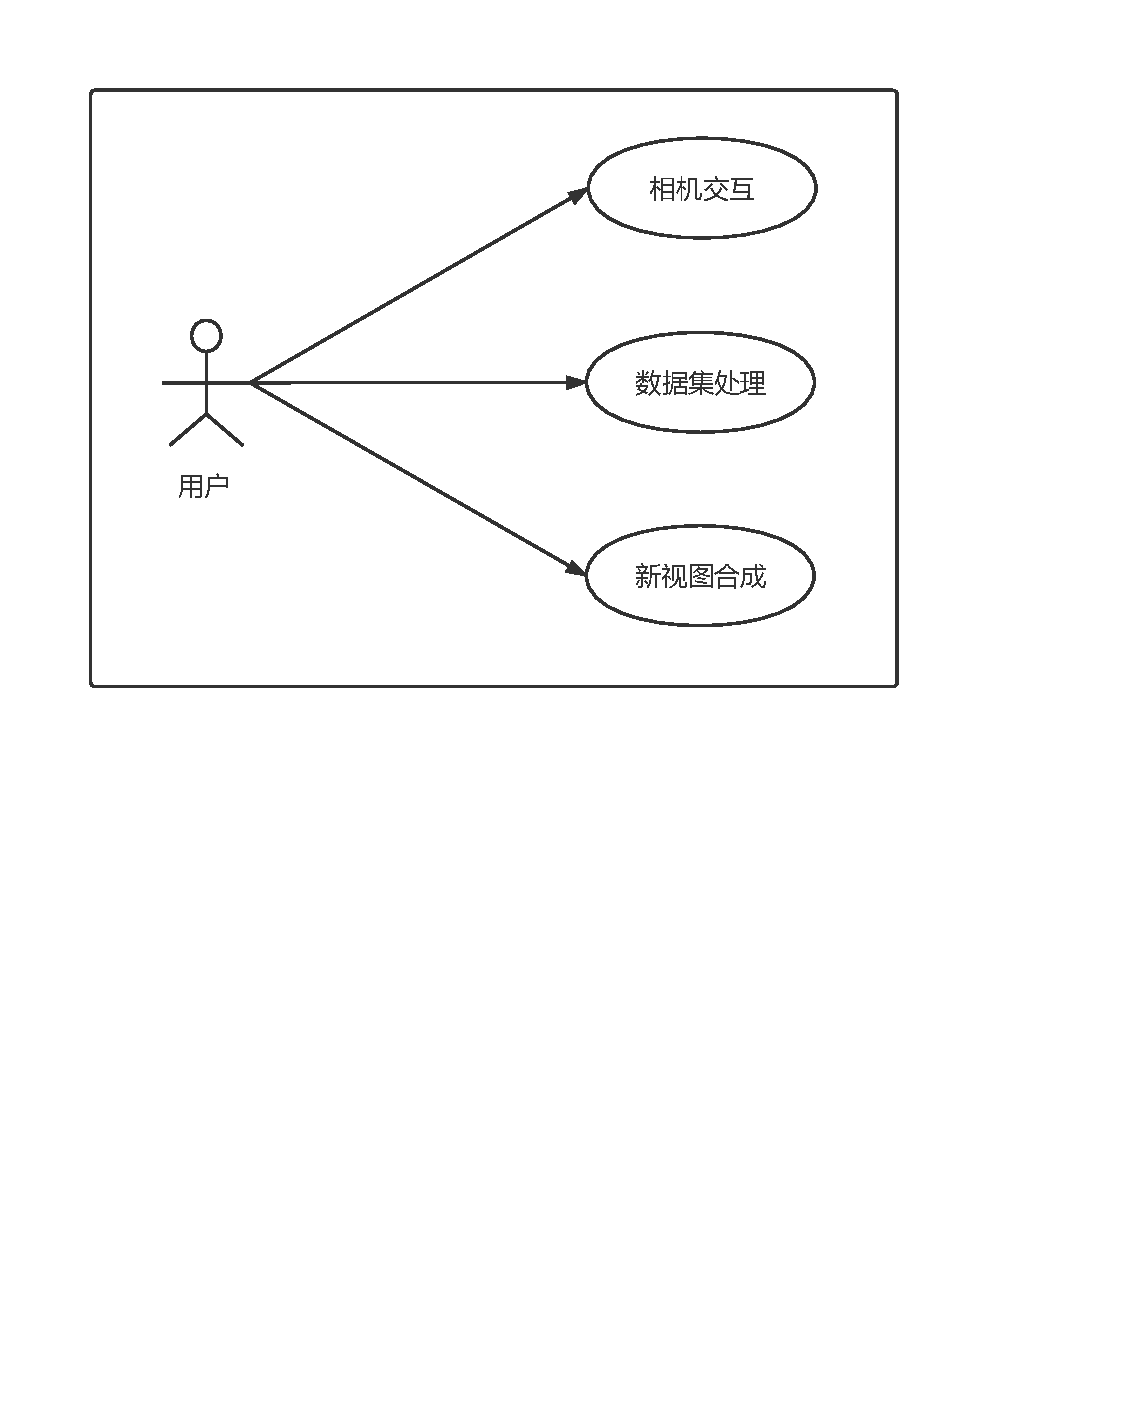
\includegraphics[width=0.55\linewidth]{figures/usercase.pdf}
	\caption{PC 客户端用例图}
	\label{fig:PCusercase}
\end{figure}

\begin{table*}
	\centering
	\small\def\arraystretch{0.91}\setlength\tabcolsep{0.05\textwidth}
	\caption{相机交互用例图User case\#1}
	\begin{tabular}{p{3.5cm}|p{8cm}}
		\hline
		用例编号 & User case\#1 \\
		\hline
		用例名 & 相机交互  \\
		\hline
		涉众及其关注点 & 用户:希望进行相机交互功能  \\
		\hline
		前置条件 & 用户启动应用 \\
		\hline
		主成功场景 & 1. 用户打开应用,点击“打开相机”按钮  \\
		& 2. 应用跳转至相机界面 \\
		& 3. 用户点击添加按钮 \\
		& 4.  当前相机画面被捕获到数据集栏并显示\\
		& 5.  用户点击“关闭相机”按钮\\
		&\quad 5a. 系统提示 “您确定要关闭相机吗?”  \\
		&\quad 5b. 系统保存用户处理结果,相机画面终止  \\
		& 6.  用户点击“退出系统”按钮\\
		&\quad 6a. 系统提示 “您确定要退出系统吗?”  \\
		&\quad 6b. 系统保存用户处理结果,整个应用退出  \\
		\hline
		拓展 & 5a. 相机关闭取消  \\	
		 & \quad 1. 交互界面保持不变  \\	
		     & 6a. 系统关闭取消  \\	
		& \quad 1. 交互界面保持不变  \\		
		\hline
		后置条件 & 应用显示相应处理结果 \\
		\hline
		发生频率 & 高 \\
		\hline
	\end{tabular}
	\label{tab:usercase1}
\end{table*}

\begin{table*}[thbp]
	\centering
	\small\def\arraystretch{1.5}\setlength\tabcolsep{0.05\textwidth}
	\caption{数据集处理用例图User case\#2}
	\begin{tabular}{p{3.5cm}|p{8cm}}
		\hline
		用例编号 & User case\#2 \\
		\hline
		用例名 & 数据集处理  \\
		\hline
		涉众及其关注点 & 用户:希望数据集处理功能  \\
		\hline
		前置条件 & 用户启动应用 \\
		\hline
		主成功场景 & 1. 用户打开应用,点击“打开相机”按钮  \\
		& 2. 应用跳转至相机界面 \\
		& 3. 用户点击添加按钮 \\
		& 4.  当前相机画面被捕获到数据集栏并显示\\
		& 5.  用户在数据集栏点击“上(下)一张”按钮\\
		& 6.  用户在数据集栏点击“删除”按钮\\
		&\quad 6a. 系统提示 “您确定删除吗?”  \\
		&\quad 6b. 系统保存用户处理结果,当前图像被删除  \\
		\hline
		拓展 & 3a. 添加数据集前未打开相机  \\	
		& \quad 1. 弹出提示框“请打开相机”  \\
		& 5a. 数据集为空  \\	
		& \quad 1. 弹出提示框“请添加图像至数据集”  \\
		& 6a. 点击取消删除或提示栏右上角$\times$  \\	
		& \quad 1. 数据集栏当前画面被保留  \\
		& 6b. 删除时,数据集为空$\times$  \\	
		& \quad 1. 弹出提示框“不可删除空数据”  \\	
		\hline
		后置条件 & 应用显示相应处理结果 \\
		\hline
		发生频率 & 高 \\
		\hline
	\end{tabular}
	\label{tab:usercase2}
\end{table*}

\begin{table*}[thbp]
	\centering
	\small\def\arraystretch{1.7}\setlength\tabcolsep{0.05\textwidth}
	\caption{新视图合成用例图User case\#3}
	\begin{tabular}{p{3.5cm}|p{8cm}}
		\hline
		用例编号 & User case\#3 \\
		\hline
		用例名 & 新视图合成  \\
		\hline
		涉众及其关注点 & 用户:希望执行新视图合成功能  \\
		\hline
		前置条件 & 用户启动应用 \\
		\hline
		主成功场景 & 1. 用户点击“计算位姿”按钮  \\
		& 2. 进度条提示计算位姿的过程 \\
		& 3. 用户点击“训练模型”按钮 \\
		& 4.  进度条提示模型训练的过程\\
		& 5.  用户点击“合成新视图”按钮\\
	    & 6. 状态提示从“待合成”到“合成中”再到“已合成” \\
	    & 7. 用户在数据集栏点击“上(下)一张”按钮 \\
		\hline
		拓展 & 1a. 计算位姿时,数据集为空:  \\	
		& \quad 1.   弹出提示框:“数据集不能为空”\\
		& 3a. 训练模型时,位姿为空:  \\	
		& \quad 1.   弹出提示框:“请先计算位姿”\\
		& 5a. 训练模型时,未训练模型:  \\	
		& \quad 1.   弹出提示框:“请先训练模型”\\		
		\hline
		后置条件 & 应用显示相应处理结果 \\
		\hline
		发生频率 & 高 \\
		\hline
	\end{tabular}
	\label{tab:usercase3}
\end{table*}

\pagebreak	
\section{系统设计}
本文提出的神经辐射场的新视图快速合成系统主要分为三个部分,包含界面层、业务层、数据层。其中,界面层主要是为用户提供可视化的应用界面以方便用户进行相应的操作。业务层提供了本系统的所有业务基本操作,包括传感器驱动、位姿估计、神经辐射场训练、新视图合成。数据层负责数据库的管理和数据的控制,通过相机获取一系列 RGB 图像,并传给业务层去处理下游任务。本文系统是基于 Windows 平台的应用,对应的 PC 客户端使用 matlab 的 App Design 工具箱实现,具体的系统架构如图~\ref{fig:symtem_design}所示。

\begin{figure}[htbp]
	\centering
	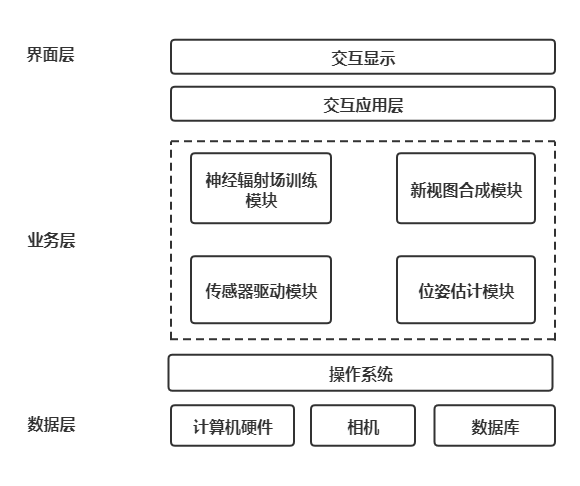
\includegraphics[width=0.75\linewidth]{figures/system_design_revised.png}
	\caption{系统功能结构图}
	\label{fig:symtem_design}
\end{figure}

\section{系统实现}
本文设计并实现的基于神经辐射场的快速新视图合成系统是基于 Windows 平台开发,算法模块和数据处理模块均是基于 C++ 语言编写,用户交互界面是基于 matlab 语言编写。C++ 和 matlab 语言之间靠动态链接库进行数据通信。由于本文使用的基于神经辐射场的新视图快速合成模型是基于 Pytorch 框架训练的,而移动传感器调用代码使用的则是 C++ 语言,为了联合开发,需要引入 Pytorch 中的 torch.jit API 用来转换成 C++ 语言支持的模型文件上。

数据处理模块的位姿估计模块是基于开源的 COLMAP 框架去估计真实世界图像的位姿的,当然这不会像合成数据集那样有绝对准确的位姿,质量这一部分势必会下降,但位姿的优化不是本文所研究的问题,在此不作过多阐述。接下来将详细介绍本文快速新视图合成算法模块的 Pytorch 模型是如何移植到 C++ 代码上的,需要使用到 LibTorch 库。

Pytorch 是 Facebook 于2007年开发的当今最流行的深度学习框架之一。它有许多优点,比如底层使用 C++ 语言编写,有类似于 numpy 的张量计算,可以用于 GPU 加速,并且支持动态图,编写调试灵活,深受深度学习开发人员的青睐。为了将 pytorch 训练好的模型能够方便地迁移到 C++ 代码中,需要使用 Pytorch 的 C++ API 模型文件 LibTorch。模型转换加载的过程如下: 

\begin{enumerate}
    \item 首先是模型转换,创建与模型相同的随机张量,使用 torch.jit.trace 模块对运算过程和权值进行跟踪和捕获,进而序列化为 LibTorch 可以加载的模型文件。
    \item 下载对应平台预编译好的 LibTorch 库,添加 include 和 lib 目录
到编译环境中。
    \item 在 C++ 代码中加载转换后的 Pytorch 模型即可调用。 
\end{enumerate}

\begin{figure}[htb]
    \centering
    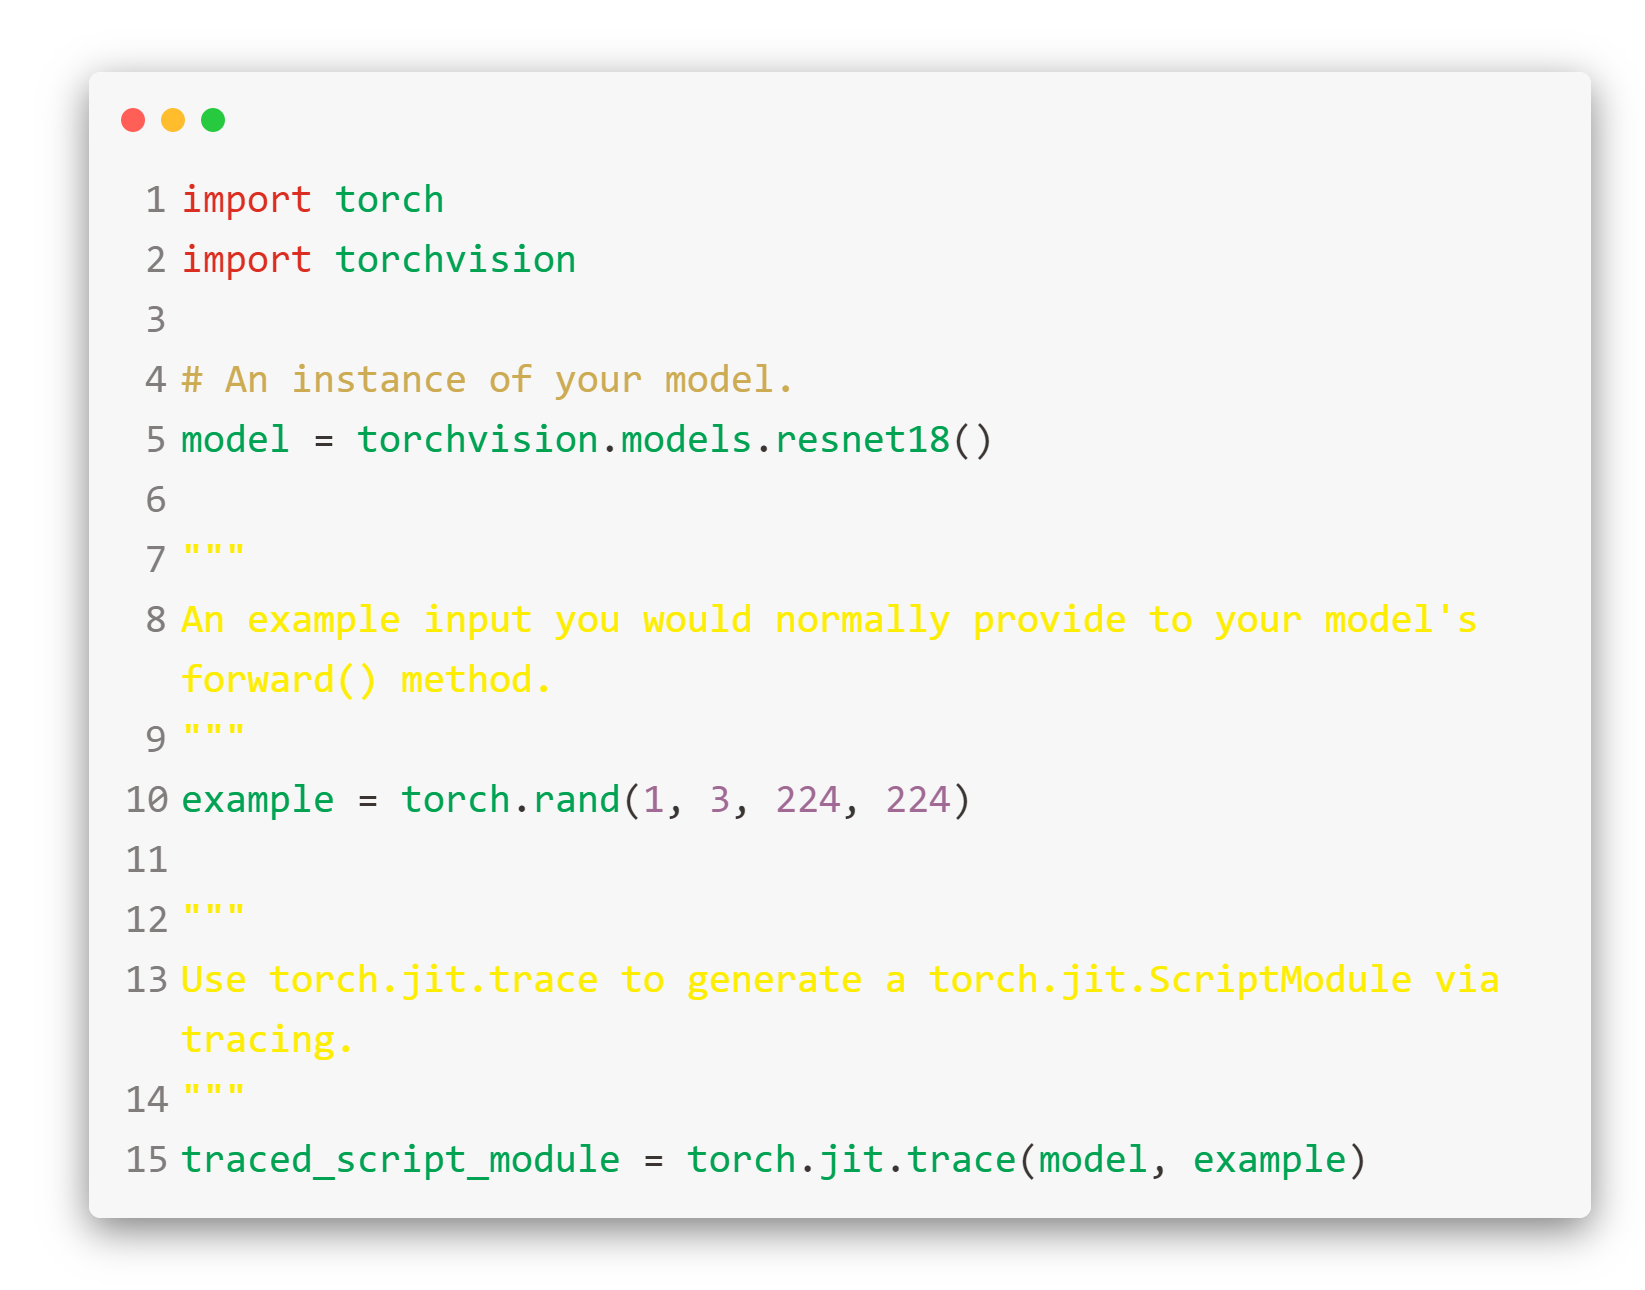
\includegraphics[width=0.98\linewidth]{figures/code-pytorch-big.png}
    \caption{Pytorch 模型的转换}
    \label{fig:code_pytorch}
\end{figure}

\begin{figure}[H]
    \centering
    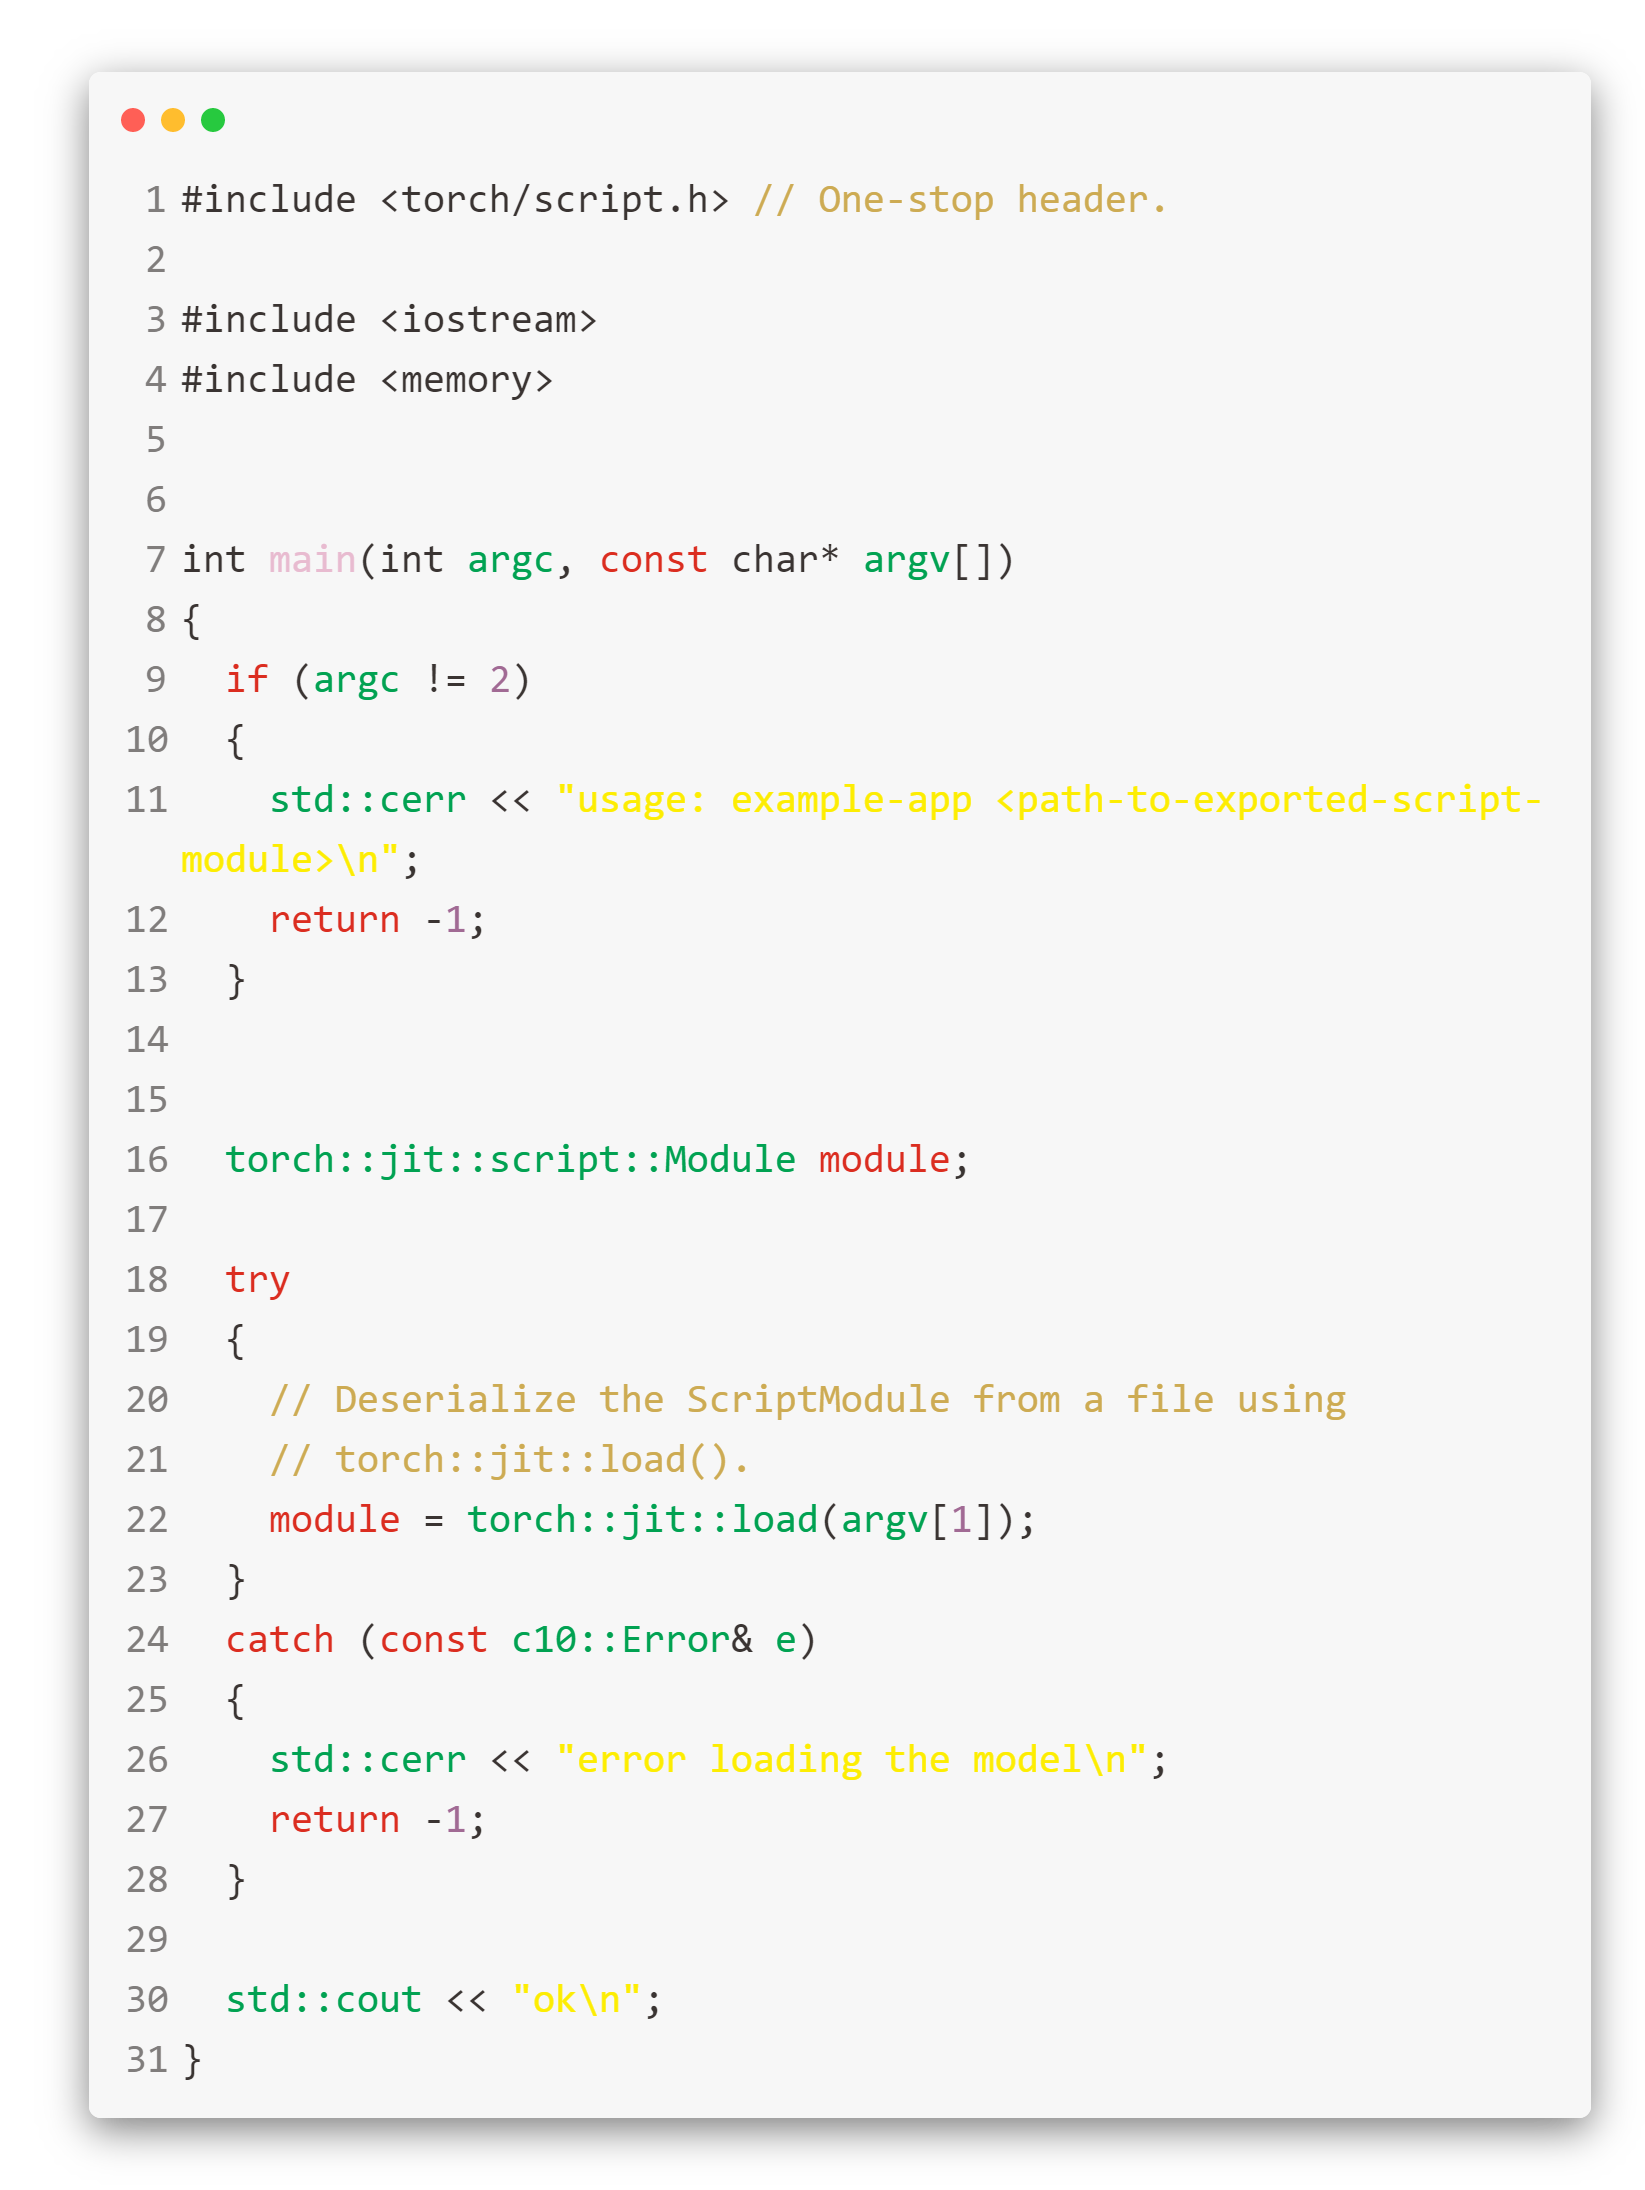
\includegraphics[width=0.98\linewidth]{figures/code-cpp-big.png}
    \caption{Pytorch 模型在 C++ 项目中的应用}
    \label{fig:code_cpp}
\end{figure}

\pagebreak

\section{本章小结}
本章主要介绍了基于神经辐射场的新视图快速合成系统的设计与实现。首先介绍了系统需求分析,包含功能性需求分析和非功能性需求分析,并展示了主要用例分析。最后阐述了此系统的基本设计架构以及将基于神经辐射场的新视图快速合成模型移植到 C++ 代码上的方法。在下一章将会详细介绍本系统的部署与展示。

\cleardoublepage
